\chapter{Background}
\label{chap:background}



\section{Ensembles}
\label{sec:ensembles}
%TO-DO: irgendwo beispielhaft erklären dass manche approaches manche sachen besser verstehen und umgekehrt, deswegen ensemble gut ist, muss maybe in die background oder introduction

When it comes to ensembling classification models, there are multiple approaches to do so. Many ensembling methods are focussed on combining homogeneous 
models, meaning a set of related models with similar architecture but different parameters or initializations. Typical methods include 
(liste an methods mit referenzen, majority vote, boosting, bagging, stacking??, CAWPE, blabla), of which i.e. (ansatz für bäume ensembles) are a typical approach to boost simple 
classifiers like trees. Homogeneous ensembles are popular, since they tend to boost the performance and robustness of a base classifier without lots 
of additional work, since the ensemble is normally created by initializing the models in different ways.
%kann der teil über diesem kommentar in die introduction?
Heterogeneous classifier ensembles on the other hand are not necessarily combinable that easily, since they usually consist of models with 
different network architectures. This can lead to results, that should be interpreted as the same, differing by large margins(synonym). Yet 
ensembles of such variety are often desirable since they offer loads of information from different perspectives or domains when done right. 
% Kann der satz weg? Combining knowledge from different domains with such an ensemble is an effective way to improve a models performance in foreign domains.
Thus to bridge this gap at the output, a common approach is to first calibrate(referenz) and then ensemble each models 
output (beweis dafür dass das normal ist). For the last combination step, all ensemble techniques suited for homogeneous ensembling can 
be applied, due to the outputs being in a comparable state then. There are also approaches to collectively calibrate the hyperparameters 
of each heterogeneous classifier while classifying(referenz). While performance varies, combining 
these models in such a way is not necessarily regarded as the highest achievable robustness, especially when the classifiers work with features or some other form of inner representation. 
This stems from the fact that the model outputs are merely a small result of larger inner representations that may focus different aspects 
of information among the inputs. Therefore in turn, you cannot obtain all relevant information that can be offered by simply calibrating the 
model outputs. A more robust approach to address that problem, would be to ensemble the aforementioned inner representations, i.e. feature maps 
and in turn train another classifier for the final meaningful output.
%----nachfolgender satz maybe raus mal gucken oder anders einbauen
Another limitation of both kinds of ensembles, being homogeneous and heterogeneous, is that all models have to actually be trained 
seperately to then utilize the different classification ouputs. This leads to a higher training time and thus also higher computational 
cost, which is desirable to be reduced in real world manufacturing firms.
It should be said that while offering a potential increase in robustness and overall performance, naturally feature level ensemble may also 
come with certain disadvantages. For instance, it is more difficult to calibrate features from the ensemble members if possible, which may 
be necessary depending on the nature of the data. An example of our context would be that certain IAD approache project their features into a 
different space to be effective, making it difficult to ensure that all features are in the same space when dealing with an ensemble. 
Moreover feature level ensembles also are vulnerable to and reliant on the quality of the input features. This makes the decision on where 
to cut off the base models very important.
%-------
The robustness and efficiency has been demonstrated in \cite{EnsembleHeller2023}. The authors utilize a feature level ensemble of multiple 
convolutional neural networks with different architectures and tasks to improve inference speed and accuracy in plant disease detection.
Heller et al.(Heller referenz) show that cutting off several, potentially heterogeneous, classifiers after a couple of network layers and ensembling the 
resulting feature maps yields firstly a significant improvement in training time compared to classical output ensembles. This stems from 
the fact, that all base classifiers of the ensemble only have to be trained once for every following training approach. During this the 
model still stays compact(zitat aus ensemble paper markieren), giving it an memory usage advantage over many supervised approaches. 
Moreover they compared the performance of different ensemble combinations with conventional 
output ensembles via the softmax function and reported in all cases no significant drop in performance. In cases where this approach allowed for 
different inputs via multispectral cameras(zitat markieren) there even was a similar performance of this ensemble to other state of the 
art ensembles visible. Keeping in mind the compactness of this new ensemble model combined with an equal performance and possible 
increased robustness, as argued prior, it is a promising ensemble approach for this work.
To obtain ensembled feature maps the paper proposes to bring all feature maps to the same sizes using bilinear interpolation. Since 
it is not necessarily desirable to keep every available feature map, as this would create inputs with way too many features, the amount of feature 
maps is reduced using principle component analysis(PCA). This allows for the ensemble to focus only on the most important features, while maintaining 
an equal amount of maps as if it were composed of a single classifier. To be more specific Heller et al. \cite{EnsembleHeller2023} introduced two different 
approaches to perform this ensemble. The first is a global transformation block as seen in figure xyz(figure mit global transformation block). 
Here the features are first all resized to the same dimensions and then connected along their channels through a concatenation layer.
Afterwards PCA is applied along the channel dimension to obtain a result with N remaining feature maps, where N can be adjusted for ones 
needs. This method offers the advantage of efficiency, as PCA is only run once per feature ensembling, and may be applied when there is 
an almost even number of feature maps per classifier with same input representations(erklärlicher schreiben?). Yet this approach is also 
prone to a couple disadvantages. If the different input data is collected from fundamentally different sources, there may be a significant 
loss of information when globally applying PCA. Furthermore this approach cannot be balanced when confronted with classifiers with large 
discrepancies in channel number. If the amount of feature maps from one classifier completely predominates, there is a high likelihood 
that most feature maps that are selected are from this classifier, if not all.
To combat this at a cost of lesser efficiency Heller et al. also introduced a second approach, namely the independent transformation block, 
visualized in figure xyz. 
This procedure is only differing in the sequencing of the actions. Therefore PCA is firstly applied to every set of feature maps, keeping 
a certain number of feature map components per classifier. They are then all resized to the desired dimensions and concatenated through 
the concatenation layer. This sequencing allows for maximum information preservation through individual PCA and also to predefine the number 
of feature maps to be kept per classifier, preventing larger imbalances.



\section{Methods of Anomaly detection}
\label{sec:IADcategs}
Over the last years a great amount of different approaches to solving IAD have been published. In order to compare different anomaly detection methods, categorizing them with respect to different 
aspects serves a better comparative analysis in regards of strengths and weaknesses.  It also helps gain a better understanding of the different approaches in the global IAD context and
is useful detect possible patterns in performance correlated to categories. This obviously also holds true for IAD approaches. Survey papers like (namen nennen) \cite{Xie_2024benchmarking} 
\cite{liu2024deep} primarily compare but also categorize IAD approaches, leading to the conclusion that there are effective and generally applicable ways to group certain approaches, as 
visualized in Figure xyz. Here it has to be said that the following categorizations naturally are a generalization, as there may be different niche settings or even approaches who combine multiple categories.
\newline
The first distinction relevant to our work is between supervised and unsupervised settings. Current deep learning approaches that have established themselves as state of the art in image anomaly detection 
are almost exclusively unsupervised approaches. This partially stems from the fact 
that in practical situations, anomalous images occur far less than normal images, hence the word "normal". This is especially true in industrial settings, due to the high performance of 
production sites nowadays. Therefore if one were to consider using a classical supervised learning approach to detect anomalies, either a strong class imbalance or a nonrepresentative class 
distribution would constitute a problem. While there are some solutions for this, they often either do not suffice for imbalances of this magnitude or far to resource extensive. To overcome 
these issues, some supervised approaches \cite{Chu_2020supervised} operate in a few-shot setting which limit the training data amount needed for proper training. Nevertheless as the focus on 
unsupervised IAD methods in current research persists, 
this work will also restrict itself to such approaches. This also facilitates the execution of the ensemble approach presented in chapter \ref{chap:method}(methods).
\newline
Looking into the unsupervised anomaly setting, the next important distinction is between reconstruction based approaches and representation based ones. They differ in the sense, that the former 
are comparing the distances between two images and the latter measure distances between feature representations. \newline
Reconstruction approaches first learn to reconstruct the objects given in the input images. This is done by feeding the network normal train data, aswell as noisy data. Noisy data are are 
which are altered by methods like gaussian noise(rephrase), although the exact noise application is depending on the specific approach. During testing, after having successfully learnt to 
reconstruct anomaly free images, the method is then given an input image, reconstructs it and compares both images using some sort of distance measure. This process is also depicted in figure xyz. 
Representation approaches on the other hand use feature embedding methods to obtain feature representations of images and compare those. As shown in figure xyz, during training the model is 
learning to correctly extract features of input images. When given an anomalous sample during testing, the model then also extracts the features from the input data and compares those to its 
prior feature level representations of the class object. A decision is then made aswell using a distance measure.
Both classes of IAD methods have shown to produce state of the art results. Yet currently more approaches are representation based \cite{liu2024deep} as they have shown SOTA performance more 
consistently. Nevertheless it is reasonable to focus on both kinds of IAD, as they may excel at different regions of anomaly detection and evaluation criteria. Namely reconstruction methods are 
often showing a better performance at pixel level anomaly detection in comparison to feature embedding/representation methods, as their principle is based on pixelwise comparisons of input 
and reconstructed data.
\newline
Again, looking at the representation based approaches, some distinctions can be made on exactly how the method implements a representation based procedure.
The main approaches in this category are ones featuring a memory bank, teacher-student architecture, distribution map and ones employ a one-class classification strategy. The characteristics of 
each strategy are visualized in figure xyz. The subcategory of 
memory bank denotes the procedure to store feature representations, that are extracted from training images, into a data collection structure. This structure is then used to compare new 
features from input images to the stored ones to form a decision. Memory bank approaches offer the upside of little training time and quick construction, yet the usually suffer from high memory 
usage and costly inference, due to the feature representations being stored into memory. Some papers have addressed this problem. Famously patchcore \cite{patchCore2022} introduced a coreset-subsampled 
memory bank, greatly improving on said bottlenecks and setting precedent for more efficient memory bank approaches. Teacher-student architectures reference the use of two networks for anomaly detection. 
This architecture has also been one of the more effective ones and its performance greatly depends on factors like the selection of the teacher model and way 
of knowledge transfer between the two networks. Here the teacher model is usually a pretrained 
backbone, that transfers knowledge onto the student model during training time, whereas the student model is simultaneously learning representations from the teacher model aswell as learning 
how to represent the input data by itself. During testing, the extracted features of teacher and student are compared, which would then be similar for normal images but have larger differences 
when presented an anomalous data point.
Next, distribution map approaches try to map the features from their original distribution into a more suitable one. This vastly facilitates a identification of anomalous features as shown in 
figure xyz. Such an approach requires a method to map the features between distributions. Often times a variation of normalizing flow is utilized for this \cite{liu2024deep}. 
Normalizing flows as a class of generative models \cite{Kobyzev_2021normalizingflowexplanation} are advantageous for transforming probability distributions because they provide a flexible 
framework to model complex distributions and efficient sampling. This enables accurate distribution mapping aswell as sampling. 
Lastly, one-class classificaiton is 
somewhat similar to a distribution mapping approach. The key difference is that the latter maps features into a desired distribution and the former focusses on finding boundaries between normal 
and anomalous features. To efficiently do that, features are projected into a suited space using a network. To learn an accurate boundary, the approaches generate fake anomalous features to 
then differentiate from normal ones. This method greatly relys on the the quality of generated features and as such may be variyngly effective. A typical approach for generating fake samples 
in this works context is with the use of gaussian noise \cite{liu2023simplenet}.
\newline
Circling back to reconstruction based methods, they also can be parted into subcategories. Here the most predominating one is the use of autoencoders to obtain a generated image. Many 
reconstruction approaches make use of typical AE encoder and decoder structures. They are mainly seperated by the method of resolving differences between the input image and the reconstructed one. 
While there are too many difference evaluation approaches to name, DRAEM \cite{Zavrtanik_2021DRAEM} can be named here as one of the most famous reconstruction autoencoder approaches. It uses 
the output of the reconstructive network in combination with the original image as the input for a discriminative subnetwork and achieves very good results and demonstrated a nearly equal effectiveness 
of reconstruction based methods to representation based ones.(nachteile von DRAEM/AE nennen)
Another, albeit less popular, approach in this category would be the use of GAN architectures/concepts to try and solve the detection problem. While we don't cover the basic principles of GANs in 
this chapter, GANs applied in IAD may still suffer the same disadvantages of regular ones, which include training instability, high computational demand and a higher difficulty of correct training and 
evaluation. Hence the use of GANs for IAD is not commonly seen, although the nature of them may promise more realistic and higher quality training data than other approaches.
Another kind of reconstruction based IAD involves the use of transformer structures. They allow for good caputiring of spatial relationships and long distance feature extraction \cite{xie2020benchmarking},
making them useful for not only structural but also logical anomaly detection. Papers like \cite{You_2023transformer} make use of transformers for feature reconstruction and as they are very 
limited in reconstructing anomalous features well, making for an easy distinction. They show in their experiments that their approach ADTR is able to outperform all shown baselines, including 
a variety of different autoencoder apporoaches.
Finally there also exists an approach that has been gaining popularity lately: the usage of the diffuion model \cite{ho2020denoisingdiffusionOG}. Papers like \cite{Wyatt_2022diffusionfirstapproach} 
leverage the models ability to capture complex dependencies to detect anomalies in IAD, and other papers \cite{zhang2023diffusionaddiffusionmodern} further improved its efficiency by speeding up 
the denoising process.
\newline
After carefully categorizing the important classes of unsupervised IAD, it is now discernible how many different approaches towards anomaly detection exist, and may yield differnt merits. 
Below(maybe sections auzählen/zitieren?) we further elaborate on a few select IAD approaches from different categories who were utilized for the MVTecAD LOCO performance analysis or the ensemble 
model. 



%reconstruction methods beschreiben
%sagen welche methods vorzeige approaches in den einzelnen categorien sind(vllt)
%sagen welche kategorien wir ausgewählt haben zum testen und dass diese genauer ausgeführt sind in den according sections
%bissi vor und nachteile der ansätze reinstreuen



\section{Datasets}
\label{sec:datasets}
The datasets used in image anomaly detection are scarce, especially when it comes to anomaly detection in a manufacturing setting. There are many datsets and approaches that specialize on certain materials \cite{FabricDataset_Tsang_2016} 
\cite{SteeltubeDataset_Yang_2021} \cite{magnetictiles_Huang_2018}
and often only one classs. What currently stands out as a gold standard among IAD datasets is the MVTecAD \cite{MVTEC_Bergmann_2021} dataset. The authors created it  
as a highly representative and standardized set of anomalous images along with training images. It has 15 classes from capsules to screws. Moreover the dataset provides image labels aswell as segmentation 
ground truths, making it versatile and applicable for multiple algorithms. The masks come as black and white grayscale images, while the image labels are given through its folder structure. 
Its paradigmatic structure tree can be seen in figure xy. As shown, each class contain train images, which only consist of regular examples, 
and test images. The data among the testing images is categorized by a title describing the anomaly. The ground truth folder contains 
according ground truths on a pixel level. Example images of the dataset are to be seen in figure z. They typically are of a rectangular shape and their resolutions range from 
(pixel min) to (pixel max). More specifications can be found in Bergmann et al. \cite{MVTEC_Bergmann_2021} and the whole dataset is publicly available at the official website\cite{mvtecdownload}.\newline
The MVTecAD(referenz) dataset is regarded highly among IAD papers, and has since its introduction been used in most relevant papers as a dataaset 
to benchmark the respective approaches on. This is also likely to remain the trend, since many state of the art algorithms in the recent years have primarily been benmarked on it, forcing new approaches 
to also be benchmarked on this dataset to be comparable to the current highest performance holding approaches. Despite this work focussing on manufacturing settings MVTecAD is one of only two datasets relevant to this work, 
and serves as a comparison for the performance investigation of this papers approaches on the second dataset. This is mainly due to the dataset's importance and 
its relation to the second dataset.
\newline
Later in 2022 Bergman et al. has introduced another IAD dataset that is loosely related to their original MVTecAD dataset, namely the MVTecAD LOCO dataset \cite{LOCODentsAndScratchesBergmann2022}. 
This dataset works with the same ground ideas as their original MVTecAD set, but extends the conceptual contents of the dataset by logical anomalies(neu formulieren das klingt scheiße). 
It consists of five classes: breakfast box, juice bottle, pushpins, screw bag and splicing connectors. The difference to the other dataset is that the anomalous categories for each class are only seperated into good images, images with structural anomalies 
and images with logical anomalies. As mentioned in the introduction structural anomalies are visible damages to the objects, similar to the MVTecAD dataset. Logical anomalies denote violations against arbitrary restrictions 
imposed by the authors. To illustrate this by an example: The class of pushpins represents a birds view of a compartmentised box of pushpins(see figure a). A rule added was, 
that each compartment is only to contain one pushpin. This means that if one region were to miss their contents, or contain more than one pushpin, it would constitute a logical anomaly. If on the 
other hand a pushpin would have a crooked or broken tip, it would be  labelled a structural anomaly. Structurally the differences of the 
MVTecAD and the MVTecAD LOCO dataset can be seen when comparing figures a and b, which showcases the anomaly classification, aswell as 
the method of storing segmentations. Here there eixists an image file for each anomalous ground truth area, which are mapped to the image 
by the folder name they are in. Lastly there exists a validation set in this dataset,
\newline
The addition of logical constraints opened an interesting area of research, since the high performance 
of current state of the art algorithms were only measured on structural anomalies so far. Yet it would be insightful to see if those models could also detect logical anomalies, since those also ocurr 
in real life settings, such as manufacturing settings. Another concept introduced in \cite{LOCODentsAndScratchesBergmann2022} is the 
saturated per-region overlap score, also sPRO. The metric is further analysed in setion (metrics section), but in short gives a measure 
on how well two regions overlap, while also accounting for regions overlapping in a way, that is seen as sufficient. The criterion of 
sufficiency is given by a file in the respective class, which maps a saturation score to each kind of anomaly.
Bergmann et al.\cite{LOCODentsAndScratchesBergmann2022} lastly also released a new IAD model together with the new dataset. The model uses autoencoders(bissi besser beschreiben hier). Since the source code has not been made public, 
this work refrains from using the method proposed in the paper.


\section{Model Calibration}
\label{sec:modelcalibration}
Calibration or rather confidence calibration is the process of adjusting/scaling your models ouput so that it indicates how likely it is to be correct. This is an important action, as nowadays 
models demonstrate increasingly good performance, scoring very high accuracies on classification tasks. Models that show to be correct that often, generally also have porential to be deployed in 
real world use cases, which especially holds true in IAD research for manufacturing contents. \cite{Guo_2017_tempscalingetc} reports that most modern neural networks are poorly calibrated in regard 
to their confidence. Current IAD methods investigated in this work confirm this, only returning anomaly scores devoid of any confidence indication. Correct confidence calibration can help evaluate 
models using new metrics, increase the users trust into the application and also help to decide on how to utilize the predictions of the model in ones context \cite{whyUncertaintyIsImportant}. 
\newline
\cite{Guo_2017_tempscalingetc} review multiple promising ways to calibrate the confidence of a model. The paper assumes certain components as method input. For a sample $x_i$ there exists the 
prediction probability $\hat{p}_i$ that $y_i = 1$, which is poorly calibrated. Moreover we are given the according non probabilistic output or logit $z_i$ for the input. The goal is to derive a 
well calibrated output confidence $\hat{q}_i$.
On a top level, the authors distinguish between calibrating binary classification models and multiclass 
ones. For binary models they present histogram binning, isotonic regression, bayesian binning into quantiles (BBQ) and lastly platt scaling. 
Histogram binning is a non-parametric approach and involves binning the uncalibrated prediction possibilities into distinct bins. Each bin $B_m$ is then assigned a confidence score $\theta _m$. During 
test time the models prediction probability $\hat{p}_i$ is mapped the score $\theta _m$ of the bin $B_m$ it falls into, resulting in a calibrated confidence $\hat{q}_m = \theta _m$. The 
boundaries of the bins are here chosen so that they minimize the bin-wise squared loss in accord to:
%Hier formel einfügen


Another non parametric approach is the solution with isotonic regression. This means to learn a piecewise constrant function $\mathcal{f} \ni \hat{q}_m = \mathcal{f}(x_i)$. This may serve as a 
optimized strict generalization of the histogram binning approach as the function can be written as: %formel und boundaries erwähnen
Another extension of histogram binnning would be BBQ, which marginalizers out all possible binning schemes to produce $\hat{q}_i$ (entweder zutat kennzeichen oder neu formulieren). A binning schemes 
is denoted by \cite{Guo_2017_tempscalingetc} to be a pair $(M, \mathcal{I})$, with $M$ being the number of bins and $\mathcal{I}$ a corresponding partition of $[0, 1]$ into disjoint intervals. 
%noch bissi beschreiben, kb jetzt


Lastly there is the parametric approach for binray prediction classifiers called platt scaling. This is the only approach that doesn't require the uncalibrated predicted probabilty and solely utilizes 
the classifiers' logits to infer a calibrated confidence. The approach can be summarized with fitting a logistic regression model on the uncalibrated non-probabilistic model outputs. An exemplary 
solution in the context of neural networks may be to optimize two scalar parameters $a, b \in \mathcal{R}$ so that $\hat{q}_i = \sigma(az_i + b)$ achieves an optimal fit. \cite{Guo_2017_tempscalingetc} 
stress that this method only calibrates the output after training, while the networks parameters stay fixed during this calibration aswell as thereafter.
\newline
As mentioned the paper also touches on model calibration for multi class prediction models, like certain binning method extensions or matrix and vector scalings. These will not be discussed here, 
since the problem context of this work revolves around binary classificaion methods.




\section{Metrics}
\label{sec:metrics}
Metrics are known to be an important part of developing any artificial intelligence related models. Many of them are used to infer 
different characteristics of model performance and should be used in different appropriate circumstances, depending on which aspect 
is important for the current application. Therefore, before the actual developing, one must first choose appropriate metrics 
to optimize and evaluate on later. IAD as a research area themselves has certain metrics that are the main performance evaluation tool 
across most papers. 
A collection of different metrics in this domain are displayed in table \ref{tab:metrics}, which is taken from 
\cite{liu2024deep}. Visible are well known 
ones from many other machine learning models like precision, recall, TPR, FPR and the F1-Score. These are generally applicable in most 
cases, but are not listed in any recent important papers and thus are not important for any analyses in this work. The other metrics are 
more IAD specific. By a large margin, the most important scoring standard is the AUROC. This metric is usually referenced for image level 
binary classification and gives an indication on how good the model is able to distinguish between both classes. Its calculation can be seein in 
table \ref{tab:metrics}. Moreover it can be used on a pixel level, which is also a popular approach but not utilized everywhere.
Next in importance is the per-region overlap(PRO) score or also the area under the PRO score(AU-PRO). This metric denotes the per-region overlap of two areas 
on a pixel level and can be calculated using (PRO formel hier hin, im satz rechts dann ggf bezug auf formel zeichen nehmen). The two areas 
compared are generally an image mask and the according segmentation by the model. The AU-PRO is then calculated by plotting the PRO score 
at different threholds for the segmentations, and reporting the area under the curve. This can be 
used to rate the segmentation performance of different models and is also a frequently featured metric in IAD related research. 
Related to this score is the saturated per-region overlap (sPRO) and also the according are under the curve, the AU-sPRO. This metric was 
introduced in \cite{LOCODentsAndScratchesBergmann2022} and briefly mentioned in section (dataset section). The method of deriving the sPRO 
score is shown again in equation abc, where $m$ denotes the amount of anomalous regions in an image, $A_i | i \in \{1, ... , m\}$ an anomalous 
region among them and $s_i | i \in \{1, ... , m\}$ a respective saturation threshold. $P$ is considered to be the pixels classified as anomalous 
in the target image. The sPRO score is the calculated by averaging the intersections of all predictions and ground truths of an image, 
while norming the values by the saturation threshold and proividing an upper limit of 1 per region. It is to be said that this gives a similar 
view on the segmentation performance as the PRO score, as it is a generalized form of it and can producet the same results if the saturation 
threshold would be equal to the amount of anomalous pixels per region. However, due to its cap of 1, it also rates differently large segmentations equally in cases 
where the anomalous position posesses some uncertainty. Figure xy demonstrates this behaviour in the case of a logical anomaly of the pushpin class. 
As visible, the logical anomaly consists of an empty pushpin compartment. The missing pushpin could be placed in any place of this smaller 
box for it to be valid, therefore an amount of pixels equal to the amount a visual pushpin posesses would suffice. Yet the conventional PRO score 
would keep on rising as the segmented area gets larger within the anomalous region. Due to the saturation score and limit. this is prevented 
by the sPRO metric as figure xy shows it to be already saturated once the minimum required amount of pixels is achieved. The saturation 
scores for each anomaly have to be individually set for each anomaly, and are given for the five classes of MVTecAD LOCO \cite{LOCODentsAndScratchesBergmann2022}.



\section{Anomaly Detection Methods}
\label{sec:IADmethods}
In this section we further dive into some of the IAD approaches that can be viewed as class representative to some extent. All following methods have demonstrated SOTA performance in 
at least some categories and are participants/candidates/(synonyms) in the performance study on the MVTecAD LOCO dataset. In the this work we investigated the most widely popular categories of 
IAD, namely memory bank, one-class classification, teacher-student, distribution maps, autoencoders and diffusion models.

\subsection{PatchCore}
\label{subsec:patchcore}
As the memory bank approach patchcore \cite{patchCore2022} has been chosen. It has demonstrated very high accuracy in both image and pixel level anomaly detection and set a high standard for 
performance after its release. The fundemental principle of patchcore is visualized in figure \ref{fig:patchcorearchitecture} and is according to the basic memory bank principle. First a pretrained feature extractor is used 
to retreive features of the input data. Next in this paper, the features are turned into locally aware feature patches, meaning the feature maps are cut into small fields and applied preprocessing operations like pooling to ensure 
the patches to be locally aware and also of similar dimension throughout the training. This results in patches that adhere to equation(patchcore patch equation benutztne). The effectiveness of this patchwise approach is justified with each patch, despite being small, having a large enough receptive field size to provide a meaningful anomalous context when learned. 
Before commiting the resulting patches to the memory bank, patchcore first induces coreset subsampling on the set of feature vecotrs. This ensures a reasonably small memory bank size that is 
large enough to offer good results, and yet is not to time and memory consuming when performing nearest neighbor search. As a memory bank structure, patchcore utilizes a search index by FaissNN(referenz) 
which offers the application of kNN with great speed, performance and even a desired tradeoff if necessary for a task. Since performance is the main criterion in IAD research though, this tradeoff is not 
utilized. 

\begin{figure}[ht]
    \centering
    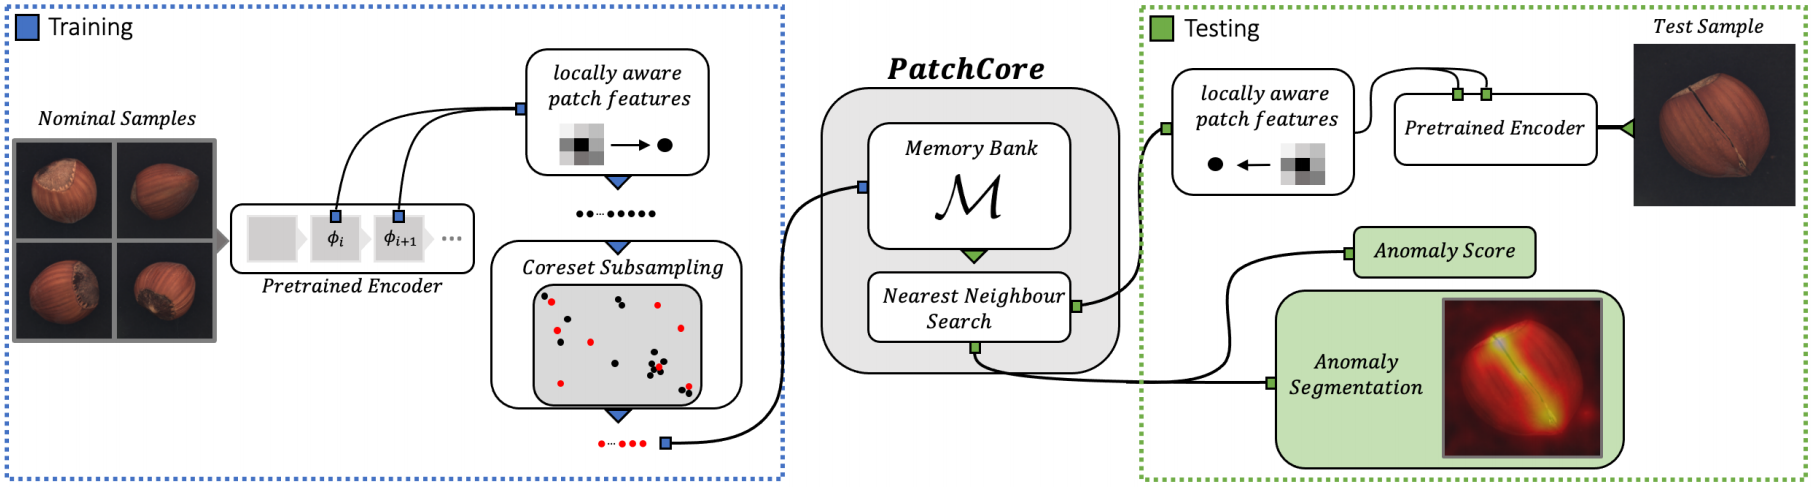
\includegraphics[width=\textwidth]{figures/pathcore_architecture.png}
    \caption{Hier korrekt zitieren}
    \label{fig:patchcorearchitecture}
\end{figure}

At test time, the input images are processed exactly like the training images were, and afterwards the model searches for the nearest neighbor of each patch, and calculates a distance measument as 
in equation xyz: %equation mit distance calculation

\begin{equation}
\label{ew:patchcoredistance}
\begin{split}
m^{test, *}, m^{*} &= \argmax_{m^{test} \in \mathcal{P}(x^{test})} \argmin_{m \in \mathcal{M}} \| m^{test} - m \|_{2} \\
s^{*} &= \| m^{test, *} - m^{*} \|_{2}
\end{split}
\end{equation}

The distance scores are then used twofold: The maximum distance in addition to a weighting relative to other neighbors distances, indicates the anomaly score on an image level. Meanwhile the patchwise distances are reshaped, 
interpolatesd and smoothed to a segmentation map for pixelwise anomaly detection.
\newline
Patchcore has greatly improved the status of prior thought slow and rarther inefficient memory bank approaches throough its subsampling approach. It moreover offers to train a model with little time 
since the only training that is really done is to fit the memory bank structure with patch vectors. Besides low training time it also requires low storage cost and offers very high and state of the art 
performance that can also be boosted using simple majority voting(checken obs nicht doch averaging war) ensembles in its paper. Its performance on the MVTecAD dataset is documented in table xyz. Yet due to its nature as a representation based approach, patchcores 
efficiency is limited by the the pretrained feature extractors acting as its backbones. This problem persists but is also approached by the paper, as they offer a implementation to train the backbone 
extractor alongside the actual training.


\subsection{SimpleNet}
\label{subsec:simplenet}
SimpleNet \cite{liu2023simplenet} is a recent one-class classification approach that has also shown to compete with other state of the art methods. Table xyz records its performance to be on the same standard as patchcore 
for most of the categories, %extra satz der es spezifiziert
Moreover it was introduced by (authors of simplenet) as a easy to use or application friendly approach, (nebensatz hier).
As a one-class classificaion or feature projection approach, SimpleNet utilizes a sub network to project extracet features into another space, to then find a decision criterion between nomral and 
abnormal features. The exact pipeline of simplenet is illustrated in figure xyz. While training, a pretrained feature extractor is used to retreive features from the input data. Here it is noteworthy, 
that SinmpleNet adopts PatchCores approach of transforming extracted features into locally aware patches. This means in figure xyz, the blue tiled pane represents features in form patch vectors 
that represent the characteristics of the image. On the basis of SimpleNet being a one-class classification approahc, the features are projected in the next step, visually at the green tiled pane. 
\cite{liu2023simplenet} conducts multiple ablation experiments on different implementations of the feature adapter. They conclude that a single fully connected layer network yield the best 
performance. The extracted features are then projected using the feature adapter, which is also simultaneously trained during the training session. Before training the discriminator, the resulting 
features are used in combination with gaussian noise to produce fake features. This is done by adding the generated noise onto the features. Afterwards the discriminator is trained by giving it 
the normal patch vectors of the input data aswell as the artificial fake features, to then learn to differentiate between them. For the discriminator, the paper reports the use of a two-layer 
MLP to be very effective. The training objective for the discriminator is composed of a truncated $l1$ loss and batchwise normalization:

%simplenet loss function

At test time the features from the input image are undergoing the described process and the projected patch vectors are given to the discriminator, resulting in a score for each patch. Similar to 
PatchCore, to generate segmentations, the scores are reshaped, bilinearly interpolated and smoothened. Also the largest score acts as the image anomaly score.

SimpleNet offers great results as to be seen in table xyz, in anomaly detection and localization. According to \cite{liu2023simplenet} its inference speed is with 79 frames per second (FPS) 
not only comparably slower that PatchCore \cite{patchCore2022} with only 10 FPS 
and PaDiM \cite{Defard_2021PADIM} (1 FPS), all being representation based approaches, but also slower than many reconstruction based approaches like DRAEM with 67 FPS. As other representation 
approaches its performance is also dependent on the quality of the backbone feature extractor.


\subsection{AST}
\label{subsec:AST}

\subsection{DRAEM}
\label{subsec:DRAEM}

DRAEM \cite{Zavrtanik_2021DRAEM} is one of the reconstruction based approaches that were selected for this work. This paper is one of the more representative ones for the reconstruction branch of 
IAD techniques. The method is based on the reconstruction abilities of autoencoders to recreate normal images from altered ones. While in recent research representation based approaches did 
show SOTA performance more often, DRAEM demonstrated that representation based methods are able to compete in the same region. Tabel xyz shows DRAEMs results on the MVTecAD dataset as reported 
in their(/authors name) paper.\newline
DRAEM utilizes two subnetworks in their anomaly detection pipeline as seen in figure xyz. The first on is the so called reconstructive sub-network and is an encoder-decoder structure. The network is trained 
to receive an image with artificial noise and reconstruct it into its original state. As the distance measurement between the reconstructed image and the original one, the second network is used, 
namely the discriminative sub-network. This network consists of a u-net (u net referenz) like architecture. Input is a channel-wise concatenation of the altereed input image and the reconstructed 
one. Since the reconstructed image is supposed to be anomaly free, the two inputs should differ to some extent, which is to be learned by the second sub-network. The network outputs a segmentation map, 
which can be used as the pixelwise anomaly detection map. Moreover the resulting map is further used for image level detection. To be interpretable, the map is smoothed by a convolution filter 
and the maximum value is taken as the image anomaly score. Reconstruction methods often utilize similarity functions such as SSIM \cite{Wang_2004SSIM} to obtain segmentation masks \cite{Zavrtanik_2021DRAEM} 
\cite{liu2024deep}. While the first 
sub-network makes SSIM as part of their loss function, the discriminative sub-network breaks free of this as it automatically learns an appropriate distance measure, making it much more robust.

DRAEM offers a exemplary good performance, robustness and moderate speed with around 67 frames per second at inference time \cite{liu2023simplenet}. Still this approach may struggle on the reconstructive 
part of its pipeline when synthesizing near-in-distribution anomalies on the original input images \cite{liu2024deep} (rausfinden was das heißt und umschreiben).


\subsection{RevDist}
\label{subsec:revdist}

\subsection{CSFlow}
\label{subsec:csflow}

CSFlow \cite{csflow2022} is one of the more robust distribution map approaches for IAD. As a distribution map approach its pipeline can be seen in figure xyz. One of the concepts that make 
approaches like CSFlow stand out of other distribution mapping methods is the feature extraction and mapping on different image scales. This cross-scale flow is using cross-convolutional 
blocks \cite{liu2024deep} to make use of context between different scales. The goal of optimization is to find out of distribution features which are assumed to have a small likelihood. 
With normalizing flow \cite{Kobyzev_2021normalizingflowexplanation} as mapping approach on a cross scale level, this makes it possible to infere likelihood information of between scales contexts, 
leading to a much more improved and robust localization of anomalies. The blocks used to map between scales 
are convolutional to preserve spatial dimensions. This method automatically results in an interpretable segmentation map at different scales. The values of the segmentation map are then used to produce an 
image score for classical anomaly detection as usual.
\newline
CSFlow has proven state of the art performance on the MVTecAD dataset like the other approaches (table xyz), and makes for precise localization on this dataset. Additionally the cross-scale flow allows 
for convenient handling of high dimensionality input with little training data \cite{csflow2022}, which has been a previously reported problem in works like \cite{Rudolph_2021badNF}.





{\SetAlgoNoLine%
\begin{algorithm}[H]
\SetKwInOut{Input}{Input}
\SetKwInOut{Output}{Output}
\SetKwFor{For}{for}{do}{end for}
\SetCommentSty{small}
\DontPrintSemicolon
% KwIn
\textbf{Input: }$\theta_1, \theta_2, \phi$ \tcp*[r]{Initial parameters}
\Indp % einruekung
$\bar{\theta_1} \leftarrow \theta_1, \bar{\theta_2} \leftarrow \theta_2$\tcp*{Initialize target network weights}
$\mathcal{D}$ \leftarrow \O \tcp*[r]{Initialize an empty replay pool}
\ForEach{iteration}{
    \ForEach{environment step}{
        $a_t \sim \pi_{\phi}(a_t|s_t)$ \tcp*[r]{Sample action from the policy}
        $s_{t+1} \sim \p((s_{t+1} |s_t, a_t)$ \tcp*[r]{Sample transition from the environment}
        $\mathcal{D} \leftarrow \mathcal{D} \{(s_t, a_t, r(s_t, a_t), s_{t+1}  )\}$ \tcp*[r]{Store the transition in the replay pool}
        }
    \ForEach{gradient step}{
        $\theta_i \leftarrow \theta_i - \lambda_{\mathcal{Q}} \hat{\nabla}_{\theta_i} J_{\mathcal{Q}}(\theta_i)$ for $i \in \{1,2\} $\tcp*[r]{Update the Q-function parameters}
        $\phi \leftarrow \phi - \lambda_{\pi} \hat{\nabla}_{\phi} J_{\pi}(\phi)$\tcp*[r]{Update policy weights}
        $\alpha \leftarrow \alpha - \lambda \hat{\nabla}_{\alpha} J_{\alpha}(\phi)$\tcp*[r]{Adjust temperature}
        $\bar{\theta_i} \leftarrow \tau \theta_i + (1-\tau) \bar{\theta}_i$ for $i \in \{1,2\}$ \tcp*[r]{Update target network weights}
        }
} 
\Indm  % undefined control seq error, but it compiles
\textbf{Output: }$\theta_1, \theta_2, \phi$ \tcp*{Optimized parameters}
\caption{Soft Actor Critic}
\label{algorithm:sac}
\end{algorithm}%
}